\documentclass[11pt, a4paper, notitlepage]{report}
\usepackage[dvips]{graphicx,color,rotating}
\usepackage{polski}
\usepackage[utf8]{inputenc}
\usepackage{pstricks}
\usepackage{lipsum}
\usepackage{titling}
\usepackage{appendix}
\usepackage{tabularx}
\usepackage[hidelinks]{hyperref}
\pretitle{
	\begin{center} 
		
\includegraphics[width=40pt,height=40pt]{graphics/znak_pk} \\ 
		 \Huge\bfseries}
\posttitle{\par\end{center}\vskip 0.5em}
\preauthor{\begin{center} \Large  KWD  \\  \LARGE\ttfamily}
\postauthor{ \end{center}}
\predate{\par\large\centering}
\postdate{\par}

\pagestyle{headings}

\author{Karolina Jeż \\Dawid Górski}

\title{\textbf{Przewidywanie odporności na ściskanie betonu}}
\date{03.01.2023}

\pagenumbering{roman} 

\begin{document}
\clearpage\maketitle
\thispagestyle{empty}
\begin{abstract}
	W projekcie zostały przedstawione wyniki badań nad trenowaniem modeli dla zbioru danych Concrete Compressive Strength Data Set. Należało przewidzieć odporność betonu na ściskanie.
	Zastosowaliśmy modele regresji liniowej, regresji wielomianowej z Polynomial Features oraz z zastosowaniem algorytmu Recursive Feature Elimination.
	Modele zostały ocenione za pomocą wartości błędu średniokwadratowego oraz współczynnika determinacji. Najlepsze wyniki uzyskano w przypadku modeli regresji wielomianowej dla danych skalowanych.
\end{abstract}

\clearpage \tableofcontents
\thispagestyle{empty}

\setcounter{page}{1}

\chapter{Wprowadzenie}
\pagenumbering{arabic}
Dane do projektu pochodzą ze zbioru danych \textit{Concrete Compressive Strength Data Set}. Składają się one z dwóch plików: \textit{Concrete\_Data.xls} oraz \textit{Concrete\_Readme.txt}.
\\ \\
W pliku \textit{Concrete\_Data.xls} znajdują się dane dotyczące 1030 próbek betonu. Każda próbka została wykonana w laboratorium i poddana testowi na wytrzymałość na ściskanie. W pliku znajduje się 9 kolumn, które opisują cechy pobranych próbek betonu. W ostatniej z nich znajduje się wartość wytrzymałości na ściskanie. Pozostałe kolumny opisują cechy próbek betonu. Wszystkie dane w pliku są przechowywane jako liczby zmiennoprzecinkowe.
\\ \\
Cechy opisujące próbki betonu stanowią:
\begin{itemize}
	\item \textbf{Cement} (component 1) -- quantitative -- kg in a m3 mixture -- Input Variable
	\item \textbf{Blast Furnace Slag} (component 2) -- quantitative -- kg in a m3 mixture -- Input Variable
	\item \textbf{Fly Ash} (component 3) -- quantitative -- kg in a m3 mixture -- Input Variable
	\item \textbf{Water} (component 4) -- quantitative -- kg in a m3 mixture -- Input Variable
	\item \textbf{Superplasticizer} (component 5) -- quantitative -- kg in a m3 mixture -- Input Variable
	\item \textbf{Coarse Aggregate} (component 6) -- quantitative -- kg in a m3 mixture -- Input Variable
	\item \textbf{Fine Aggregate} (component 7) -- quantitative -- kg in a m3 mixture -- Input Variable
	\item \textbf{Age} -- quantitative -- Day (1~365) -- Input Variable
	\item \textbf{Concrete compressive strength} -- quantitative -- MPa -- Output Variable
\end{itemize}
\\
W pliku \textit{Concrete\_Readme.txt} znajduje się krótki opis zbioru danych, tj. źródło, opis atrybutów oraz autorzy.
\section{Opis problemu}
Zadanie polega na wykonaniu modelu regresji liniowej, który będzie przewidywał wytrzymałość na ściskanie betonu na podstawie 9 cech numerycznych próbek betonu. W tym celu należy wykonać analizę eksploracyjną zbioru danych, i zdecydować, które cechy mogą zostać pominięte, oraz czy należy wykonać skalowanie danych.
\\ \\
W celu sprawdzenia czy model jest wystarczająco dokładny należy wykonać walidację krzyżową, a także zwrócić uwagę na wartość błędu średniokwadratowego oraz wariancji.
\\ \\
W celu wykonania zadania wykorzystaliśmy bibliotekę scikit-learn. Wszystkie metody zostały zaimplementowane w języku Python.
\chapter{Opis metody}
\section{Wprowadzenie teoretyczne}
W celu wykonania zadania wykorzystaliśmy kilka metod uczenia maszynowego, tj: \textbf{regresję liniową}, \textbf{regresję wielomianową}, algorytm \textbf{Recursive Feature Elimination} oraz metodę \textbf{Polynomial Features}. Na potrzeby walidacji modelu wykorzystaliśmy metodę \textbf{Cross Validation}.
\\ \\
\textbf{Regresja liniowa} jest jedną z najprostszych metod uczenia maszynowego. Polega ona na dopasowaniu funkcji liniowej do zbioru danych. Funkcja ta jest zdefiniowana wzorem:
\begin{equation}
\hat{y} = \theta_0 + \theta_1x_1 + \theta_2x_2 + \ldots + \theta_nx_n
\end{equation}
gdzie:
\begin{itemize}
	\item $\hat{y}$ -- wartość przewidywana
	\item $n$ -- liczba cech
	\item $x_i$ -- wartość cechy $i$
	\item $\theta_i$ -- parametr modelu
\end{itemize}
\\ \\ \\
\textbf{Regresja wielomianowa} jest rozszerzeniem regresji liniowej. Polega ona na dopasowaniu funkcji wielomianowej do zbioru danych. Funkcja ta jest zdefiniowana wzorem:
\begin{equation}
\hat{y} = \theta_0 + \theta_1x_1 + \theta_2x_2^2 + \ldots + \theta_nx_n^n
\end{equation}
gdzie:
\begin{itemize}
	\item $\hat{y}$ -- wartość przewidywana
	\item $n$ -- liczba cech
	\item $x_i$ -- wartość cechy $i$
	\item $\theta_i$ -- parametr modelu
\end{itemize}
\\ \\ \\
\textbf{Algorytm Recursive Feature Elimination} jest algorytmem wybierającym cechy, które mają największy wpływ na przewidywanie wartości. Bazuje on na algorytmie regresji liniowej.
\\ \\
Kroki wykonywane przez algorytm RFE:
\begin{enumerate}
	\item Zdefiniuj liczbę cech, które mają zostać wybrane
	\item Wytrenuj model
	\item Oblicz wartość błędu średniokwadratowego
	\item Usuń cechę, która ma najmniejszy wpływ na przewidywanie wartości
	\item Powtórz kroki 2-4, aż zostanie wybrana określona liczba cech
	\item Zwróć wybrane cechy
\end{enumerate}
\\ \\ \\
\textbf{Metoda Polynomial Features} jest metodą, która pozwala na wygenerowanie wielu cech na podstawie istniejących. W tym celu należy podać stopień wielomianu, który ma zostać wygenerowany. Przykładowo: w przypadku stopnia 2 każda cecha zostanie podniesiona do kwadratu, a następnie zostaną wygenerowane wszystkie kombinacje dwóch cech. W przypadku stopnia 3, każda cecha zostanie podniesiona do sześcianu, a następnie zostaną wygenerowane wszystkie kombinacje trzech cech, itd.
\\ \\
Przykład:
\begin{itemize}
	\item Stopień wielomianu: 2
	\item Cechy: $x_1$, $x_2$
	\item Wygenerowane cechy: $x_1^2$, $x_2^2$, $x_1x_2$
\end{itemize}
\\ \\ \\
\textbf{Cross Validation} jest metodą walidacji modelu. Polega ona na podziale zbioru danych na $k$ części. Następnie wykonywane jest $k$ trenowań modelu, w których każde trenowanie wykorzystuje $k-1$ części zbioru danych. W ostatnim trenowaniu wykorzystywana jest pozostała część zbioru danych. W ten sposób wyznaczane są $k$ wartości błędu średniokwadratowego. Następnie obliczana jest średnia z tych wartości.

\section{Badania symulacyjne}
Na początku programu w funkcji \textit{importData()} wczytaliśmy zbiór danych \textit{Concrete Compressive Strength Data Set}. Następnie wykonaliśmy wstępną analizę zbioru za pomocą funkcji \textit{analizeData()}.
\\ \\
\subsection{Analiza zbioru danych}
Na początku wypisaliśmy pierwsze 5 wierszy ze zbioru danych. W tym celu skorzystaliśmy z funkcji \textit{head()} z biblioteki \textit{pandas}.
\\ \\
Wynik:
\begin{center}
	\small
\begin{tabular}{|m{0.5cm}|m{1cm}|m{1cm} | m{0.5cm} | m{1cm} | m{1.4cm} | m{1.2cm} | m{1.2cm} | m{0.5cm} | m{1.2cm}|}
\hline
n & Cement & Blast Furnace Slag & Fly Ash & Water & Super\-plasticizer & Coarse Aggregate & Fine Aggregate & Age & Concrete compressive strength \\
\hline
1 & 540 & 0 & 0 & 162 & 2.5 & 1040 & 676 & 28 & 79.99 \\
\hline
2 & 540 & 0 & 0 & 162 & 2.5 & 1055 & 676 & 28 & 61.89 \\
\hline
3 & 332.5 & 142.5 & 0 & 228 & 0 & 932 & 594 & 270 & 40.27 \\
\hline
4 & 332.5 & 142.5 & 0 & 228 & 0 & 932 & 594 & 365 & 41.05 \\
\hline
5 & 198.6 & 132.4 & 0 & 192 & 0 & 978 & 825 & 360 & 44.3 \\
\hline
\end{tabular}
	\caption{Pierwsze 5 wierszy zbioru danych}
\end{center}
\\ \\
Następnie wyświetliliśmy podstawowe informacje o zbiorze danych. W tym celu skorzystaliśmy z funkcji \textit{describe()}.
\\
W wyniku otrzymaliśmy następujące informacje:
\begin{center}
	\small
	\begin{tabular}{|c|c|c|c|c|}
\hline
Nazwa kolumny & Min & Max & Odchylenie standardowe & Średnia \\
\hline
Cement & 102 & 540 & 104.50 & 281.16 \\
\hline
Blast Furnace Slag & 0 & 359 & 86.27 & 73.89 \\
\hline
Fly Ash & 0 & 200 & 63.99 & 54.18 \\
\hline
Water & 121 & 247 & 21.35 & 181.56 \\
\hline
Super\-plasticizer & 0 & 32 & 5.97 & 6.20 \\
\hline
Coarse Aggregate & 801 & 1145 & 77.75 & 972.91 \\
\hline
Fine Aggregate & 594 & 992 & 77.66 & 773.58 \\
\hline
Age & 1 & 365 & 63.16 & 45.66 \\
\hline
Concrete compressive strength & 2.33 & 82.6 & 16.70 & 35.81 \\
\hline
\end{tabular}
	\caption{Podstawowe informacje o zbiorze danych uzyskane za pomocą funkcji describe()}
\end{center}
Upewniliśmy się również, czy na pewno w zbiorze nie ma brakujących danych. Skorzystaliśmy do tego celu z funkcji \textit{isnull()}, która potwierdziła, że w zbiorze znajdują się wszystkie dane.
\\ \\
Sprawdziliśmy również dystrybucję danych w zbiorze, aby określić czy są one zbalansowane. W tym celu utworzyliśmy wykres typu \textit{distplot()} z biblioteki seaborn. Na wykresie widać, że większość danych znajduje się w przedziale od 0 do 70. Wartości wykraczające poza ten przedział są rzadkie.
\\
\begin{center}
	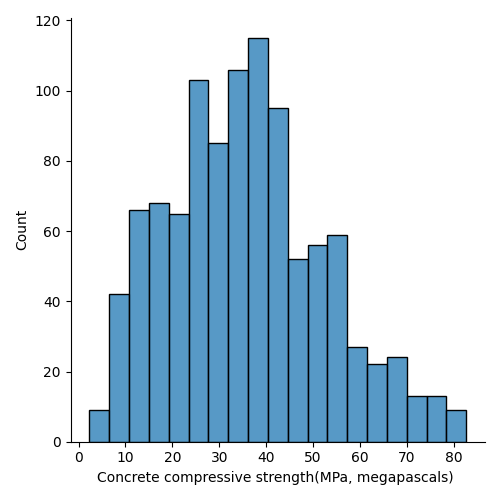
\includegraphics[width=0.9\textwidth]{graphics/data_analysis/target_distribution}
	\caption{Dystrybucja danych w zbiorze}
\end{center}
\\ \\
Za pomocą funkcji \textit{corr()} obliczyliśmy korelację między cechami. W tym celu wykorzystaliśmy bibliotekę pandas. W wyniku otrzymaliśmy następującą macierz korelacji:
\begin{center}
	\small
	\begin{tabular}{|m{3cm} | m{0.8cm} m{0.8cm} m{0.8cm} m{0.8cm} m{0.8cm} m{0.8cm} m{0.8cm} m{0.8cm} m{0.8cm}|}
\hline
 & C & B FS&FA & W & SP & CA & FA & A & CCS \\
\hline
Cement & 1 & -0.28 & -0.40 & -0.08 & 0.09 & 0.011 & -0.22 & 0.08 & 0.50 \\
Blast Furnace Slag & -0.28 & 1 & -0.32 & 0.11 & -0.04 & -0.28 & -0.28 & 0.04 & 0.13 \\
Fly Ash & -0.40 & -0.32 & 1 & -0.26 & 0.37 & 0.08 & 0.15 & -0.15 & -0.32 \\
Water & -0.08 & 0.11 & -0.26 & 1 & -0.65 & -0.18 & -0.45 & 0.27 & -0.29 \\
Super\-plasticizer & 0.09 & -0.04 & 0.37 & -0.65 & 1 & 0.02 & 0.22 & -0.19 & -0.16 \\
Coarse Aggregate & 0.011 & -0.28 & 0.08 & -0.18 & 0.02 & 1 & -0.18 & -0.02 & -0.16 \\
Fine Aggregate & -0.22 & -0.28 & 0.15 & -0.45 & 0.22 & -0.18 & 1 & -0.16 & -0.17 \\
Age & 0.08 & 0.04 & -0.15 & 0.27 & -0.19 & -0.02 & -0.16 & 1 & 0.33 \\
Concrete compressive strength & 0.50 & 0.13 & -0.32 & -0.29 & -0.16 & -0.16 & -0.17 & 0.33 & 1 \\
\hline
\end{tabular}
	\caption{Macierz korelacji}
\end{center}
\\ \\
Aby łatwiej odczytać macierz korelacji postanowiliśmy ją wyświetlić również w postaci heatmapy.
\\
\begin{center}
	\small
	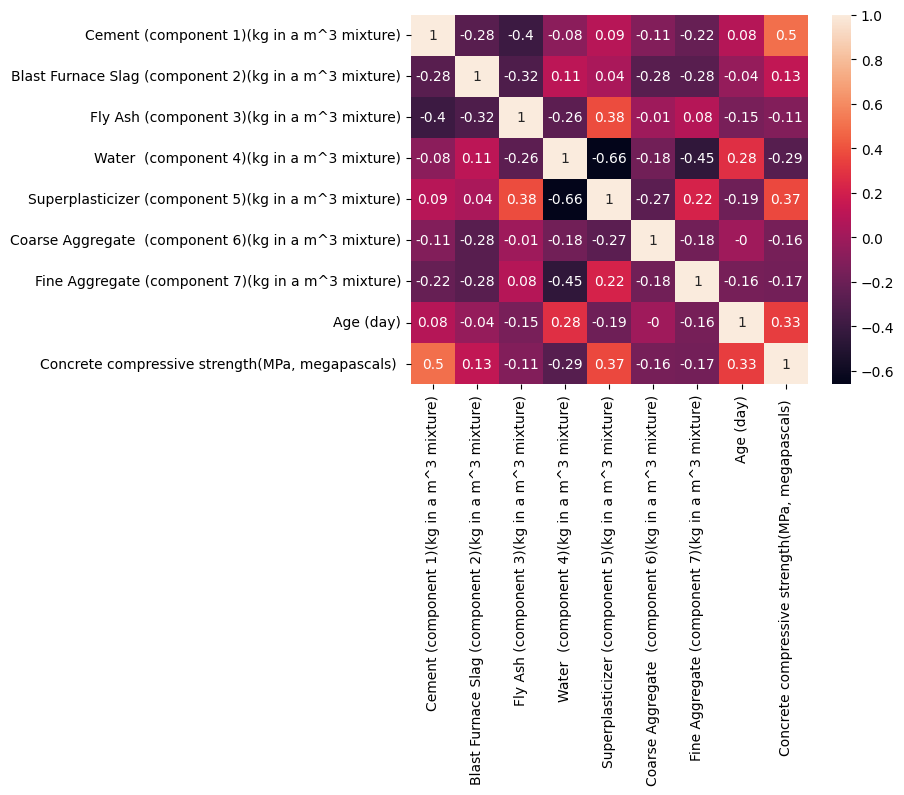
\includegraphics[width=1\textwidth]{graphics/data_analysis/heatmap}
	\caption{Heatmapa macierzy korelacji}
\end{center}
\\ \\
Wykorzystaliśmy również metodę \textit{pairplot()}, aby sprawdzić zależności między cechami.
\\
\begin{center}
	\small
	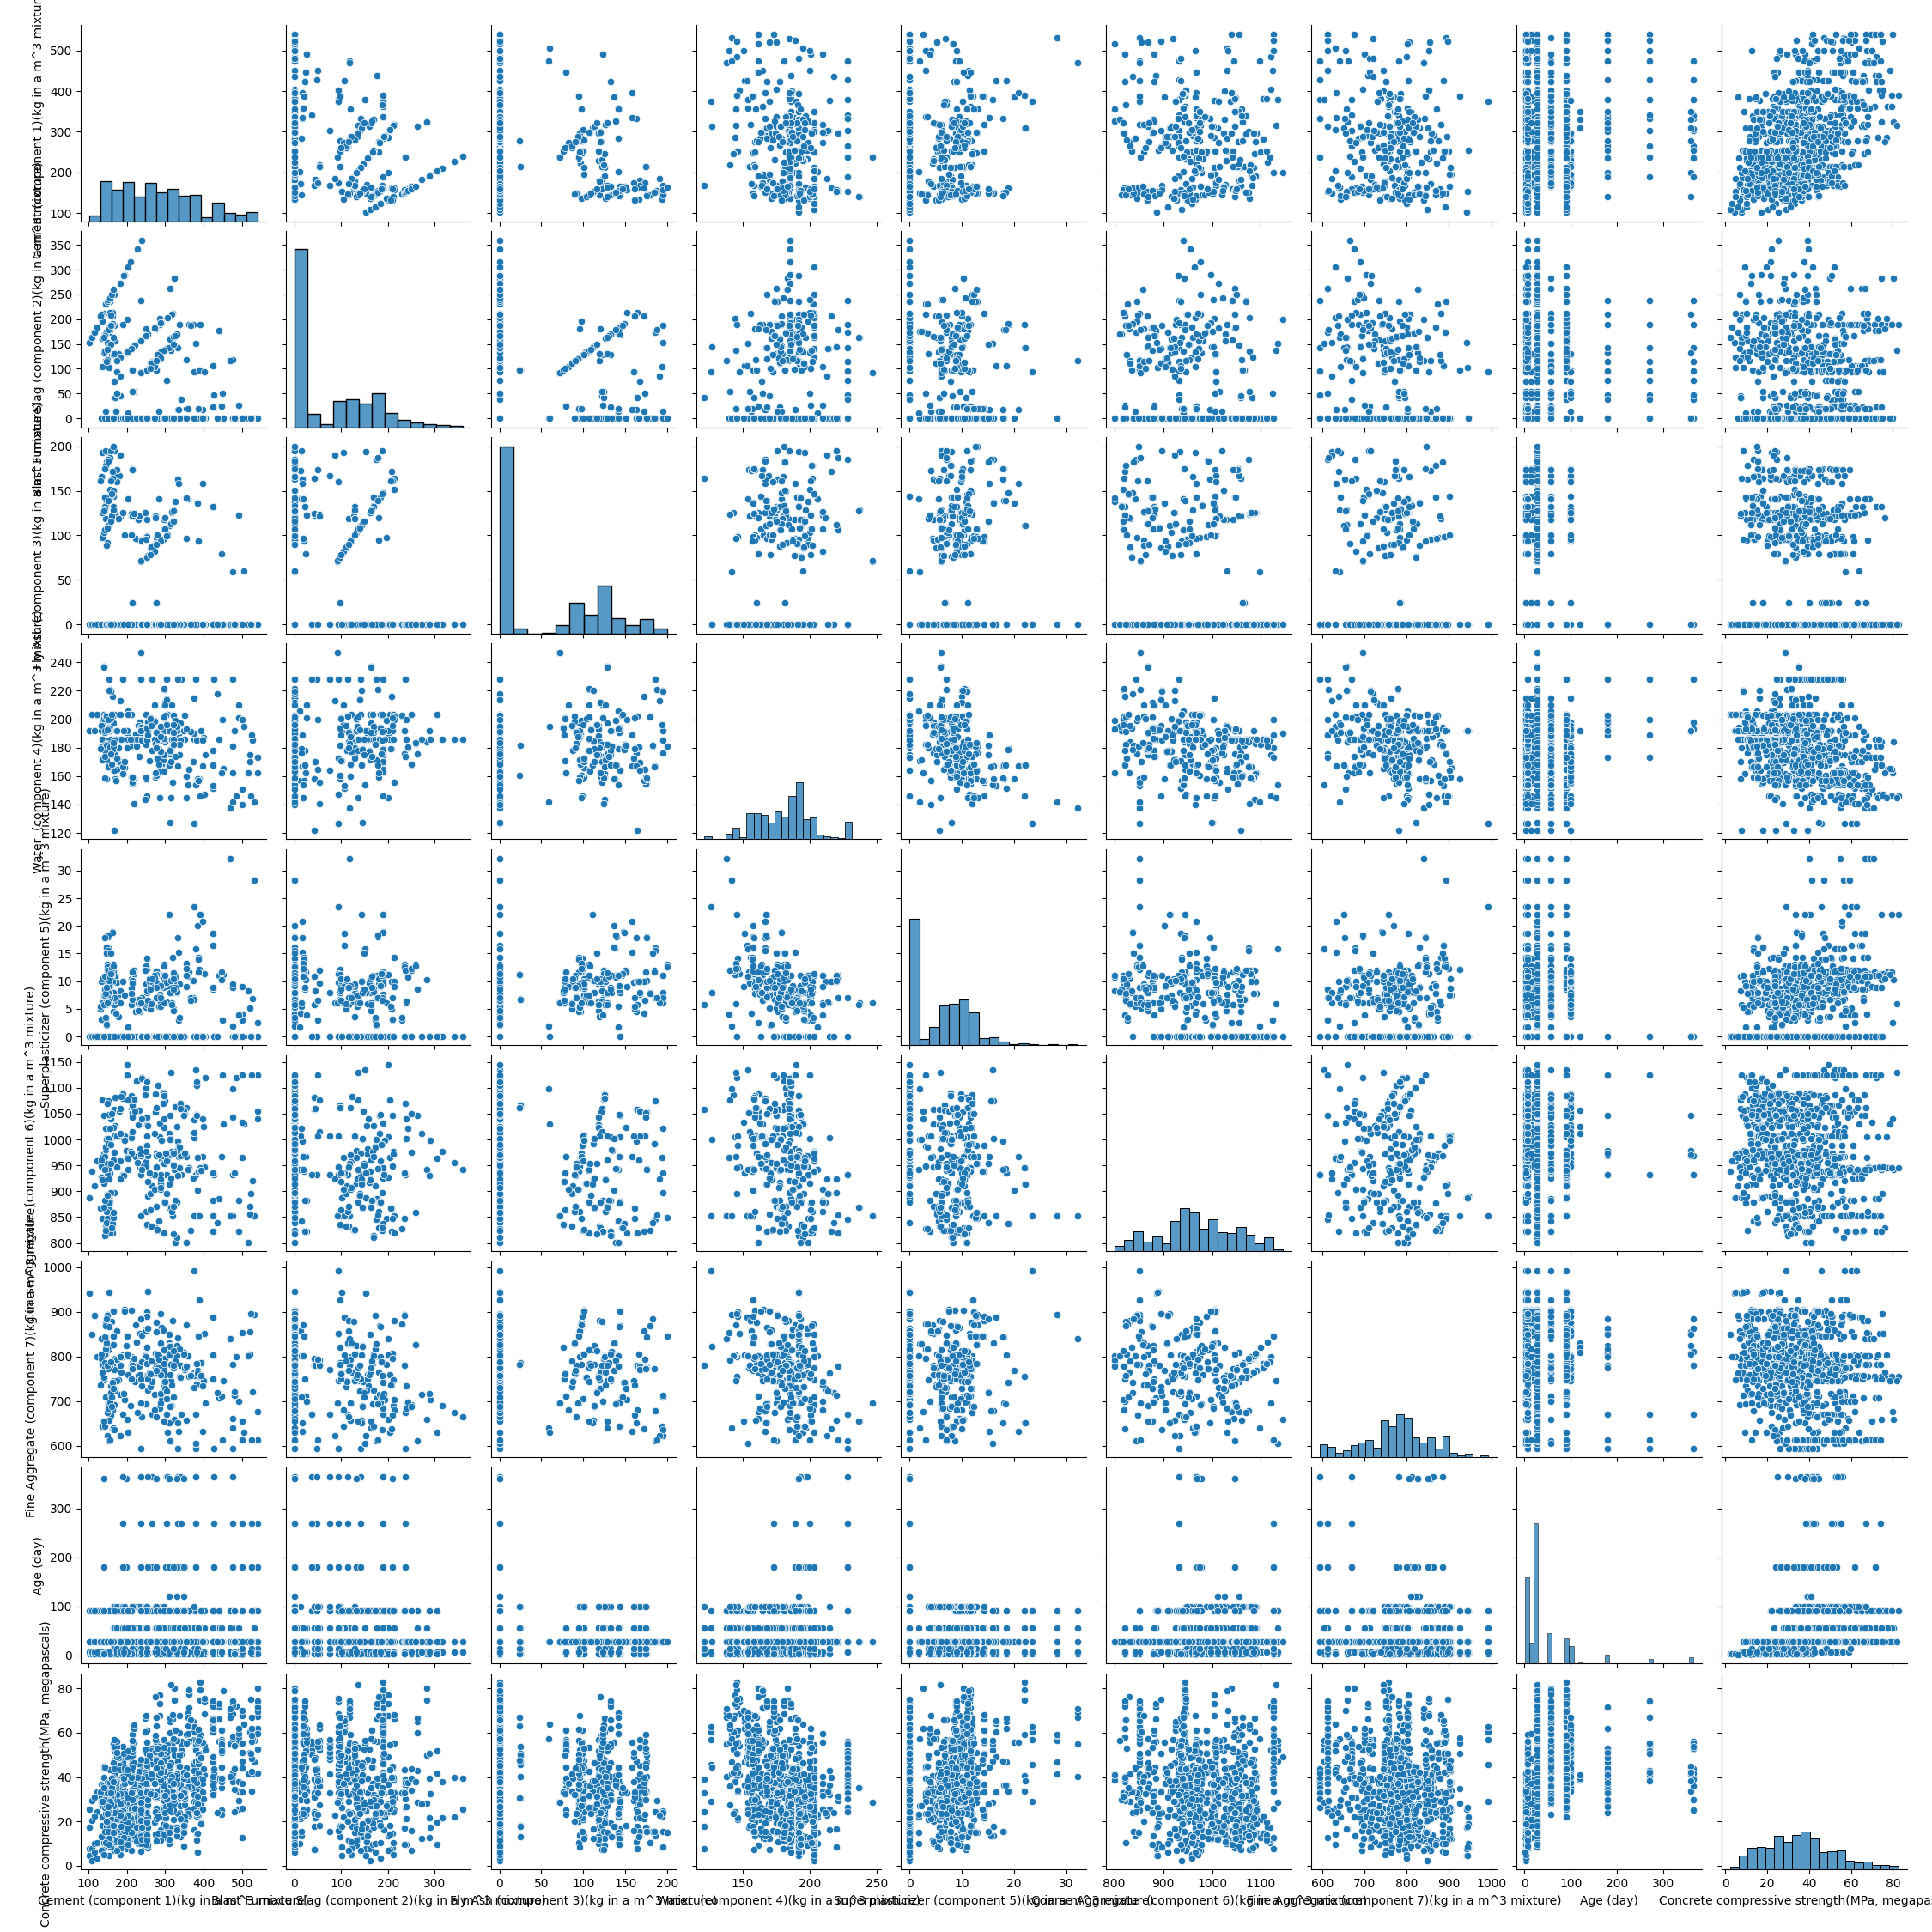
\includegraphics[width=1\textwidth]{graphics/data_analysis/pairplot}
	\caption{Wykresy zależności między cechami}
\end{center}
\\ \\
Na podstawie macierzy korelacji, heatmapy oraz wykresu zależności między cechami można stwierdzić, że cechy nie są mocno skorelowane.
W naszym przypadku zmienna najbardziej skorelowana z Concrete compressive strength (target) to Cement. Wartość współczynnika korelacji wyniosła 0.5.  \\
Warto zwrócić uwagę na cechy Water oraz Superplasticizer, które są silnie negatywnie skorelowane (-0.66)
\\ \\
W celu sprawdzenia, czy w zbiorze występują wartości odstające, wykorzystaliśmy funkcję \textit{boxplot()}. Na wykresie widać, że w zbiorze występują takie wartości w przypadku 7 kolumn.
\\
\begin{center}
	\small
	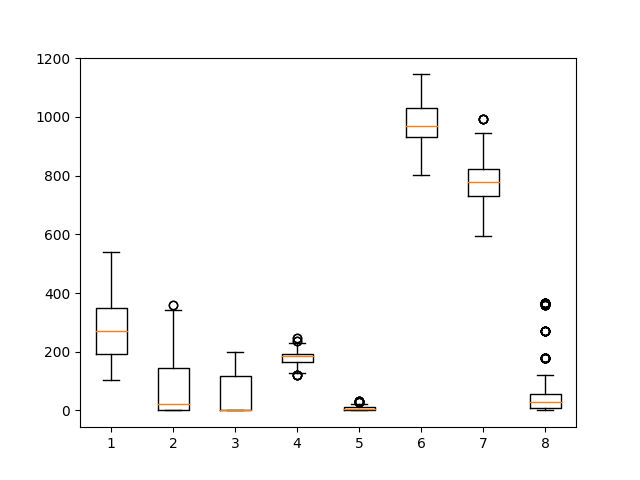
\includegraphics[width=0.9\textwidth]{graphics/data_analysis/boxplot}
	\caption{Wykres typu boxplot}
\end{center}
\\ \\
W celu sprawdzenia, czy dane są w rozkładzie normalnym, wykorzystaliśmy funkcję \textit{probplot()}.
\\
\begin{center}
	\small
	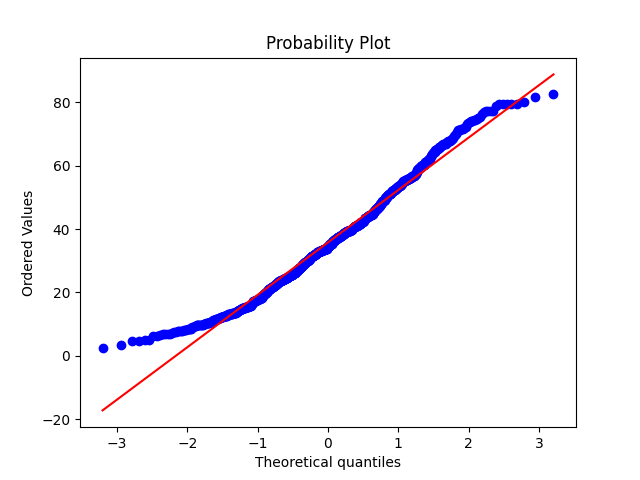
\includegraphics[width=0.9\textwidth]{graphics/data_analysis/probplot}
	\caption{Wykres typu probplot dla rozkładu normalnego}
\end{center}
\\ \\
Funkcję \textit{probplot()} wykorzystaliśmy również do sprawdzenia, czy dane są w rozkładzie log-normalnym. Jednak ta skala okazała się być gorsza od normalnej (widać to na wykresie poniżej).
Można to wywnioskować z tego, że wykres jest bardziej rozproszony, gdzie w przypadku normalnego rozkładu wykres jest bardziej skupiony wokół prostej, co oznacza, że dane powinny być dobrym materiałem do trenowania modeli regresji liniowej.
\\
\begin{center}
	\small
	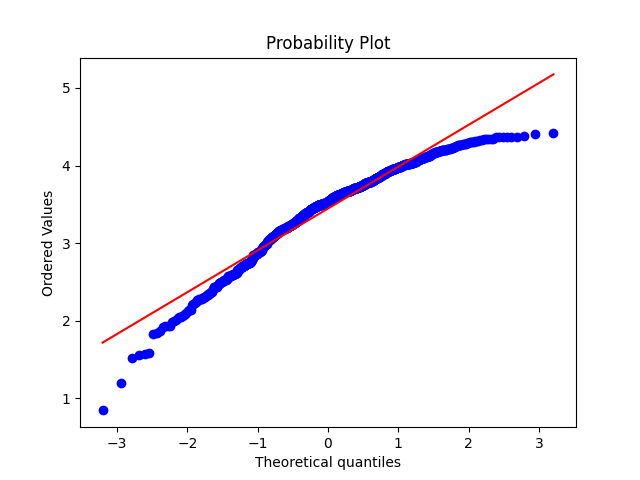
\includegraphics[width=0.9\textwidth]{graphics/data_analysis/log_probplot}
	\caption{Wykres typu probplot dla rozkładu log-normalnego}
\end{center}
\\ \\
\subsection{Przygotowanie danych}
W celu przygotowania danych do modelowania postanowiliśmy:
\begin{itemize}
	\item przeskalować dane
	\item podzielić zbiór na zbiór treningowy i testowy
	\item wybrać najlepsze cechy
	\item wygenerować dodatkowe cechy
\end{itemize}
\\ \\
W celu przeskalowania danych wykorzystaliśmy bibliotekę sklearn. Wykorzystaliśmy klasę \textit{StandardScaler}, która przeskalowuje dane do rozkładu normalnego. W celu przeskalowania danych wykorzystaliśmy funkcję \textit{fit\_transform()}.
\\ \\
W celu podziału zbioru na zbiór treningowy i testowy wykorzystaliśmy funkcję \textit{train\_test\_split()} z biblioteki sklearn. Funkcja ta dzieli zbiór na zbiór treningowy i testowy w podanych proporcjach.
\\ \\
Wybór cech wykonywany jest za pomocą klasy \textit{RFE} z biblioteki sklearn (funkcja \textit{fit()}).
\\ \\
Generowanie dodatkowych cech wykonywane jest za pomocą klasy \textit{PolynomialFeatures} z biblioteki sklearn (funkcja \textit{fit\_transform()}).
\\ \\

\subsection{Schemat symulacji}
W celu eksperymentu postanowiliśmy wytrenować modele według następujących reguł:
\begin{itemize}
	\item trenowanie modeli wykonujemy zarówno na zbiorze oryginalnym jak i na zbiorze po przeskalowaniu
	\item w każdym przypadku trenujemy 3 rodzaje modeli: za pomocą regresji liniowej, regresji wielomianowej z zastosowaniem Polynomial Features oraz algorytmu Recursive Feature Elimination (RFE)
	\item każdy rodzaj modelu trenujemy dla różnych rozmiarów zbioru treningowego (20, 30, 40, 50\%)
	\item w przypadku zastosowania Polynomial Features trenowane są modele o stopniu wielomianu 2, 3 oraz 4
	\item w przypadku zastosowania RFE trenowane są modele dla różnej liczby cech (od 5 do 14), dla stopnia wielomianu 2 (z naszych obserwacji wynika, że stopień wielomianu 2 jest najlepszy)
	\item dla każdego modelu obliczane są następujące metryki: średni błąd kwadratowy, współczynnik determinacji (R2), waliacja krzyżowa (Cross Validation) dla cv od 2 do 4
	\item każdy model ma generowaną unikalną nazwę
	\item dla modeli trenowanych na zbiorze oryginalnym i przeskalowanym wybierany jest po jednym najlepszym modelu (na podstawie wartości średniego błędu kwadratowego, współczynnika determinacji oraz walidacji krzyżowej)
	\item wartości metryk dla każdego modelu zapisywane są do pliku csv (osobno dla zbioru oryginalnego i przeskalowanego)
	\item dla każdego modelu generowany jest wykres porównujący wartości rzeczywiste z wartościami przewidywanymi
	\item wykresy zapisywane są do plików png o nazwie odpowiadającej nazwie modelu
\end{itemize}
\\ \\
Schemat nazewnictwa modeli:
\begin{center}
\textbf{[skrót\_metody]\_[parametry\_modelu]\_[s/ns]}
\end{center}
\\ \\
Gdzie:
\begin{itemize}
	\item skrót\_metody - akronim metody użytej do trenowania modelu, są to odpowiednio: LR (dla regresji liniowej), PR (dla regresji wielomianowej), RFE (dla Recursive Feature Elimination)
	\item parametry\_modelu - parametry modelu: \begin{itemize}
		\item s - rozmiar zbioru treningowego
		\item d - stopień wielomianu
		\item nf - liczba cech
	\end{itemize}
	\item s/ns - oznaczenie danych (ns - dane oryginalne, s - dane przeskalowane); znajduje się na końcu nazwy modelu
\end{itemize}
\\ \\
Przykładowe nazwy modeli:
\begin{itemize}
	\item LR\_s\_0.2\_s - regresja liniowa, 20\% zbioru treningowego, zbiór skalowany
	\item RFE\_d\_2\_nf\_6\_s\_0.5\_ns - Recursive Feature Elimination, stopień wielomianu 2, 6 cech, 50\% zbioru treningowego, zbiór nieskalowany
	\item PR\_d\_3\_s\_0.3\_s - regresja wielomianowa, stopień wielomianu 3, 30\% zbioru treningowego, zbiór skalowany
\end{itemize}
\\ \\
Schemat zapisu metryk do pliku csv:
\begin{itemize}
	\item nazwa plików to \textit{non-scaled\_results.csv} i \textit{scaled\_results.csv} odpowiednio dla zbioru oryginalnego i przeskalowanego
	\item dane modeli zapisywane są w kolejnych wierszach
	\item nazwy kolumn to: \begin{itemize}
		\item name - nazwa modelu
	   \item mean - bład średniokwadratowy
	   \item variance - wariancja
	   \item cv2 - walidacja krzyżowa dla cv=2
	   \item cv3 - walidacja krzyżowa dla cv=3
	   \item cv4 - walidacja krzyżowa dla cv=4
	   \end{itemize}
\end{itemize}
\subsection{Wyniki symulacji dla danych bez skalowania}
Na podstawie wygenerowanych modeli wybraliśmy trzy najlepsze z nich dla zbioru oryginalnego. Są to:
\begin{enumerate}
	\item Model regresji wielomianowej stopnia 2 dla 30\% zbioru treningowego
	\item Model regresji wielomianowej stopnia 2 dla 50\% zbioru treningowego
	\item Model z wykorzystaniem RFE stopnia 2 o 8 cechach dla 30\% zbioru treningowego
\end{enumerate}
\\ \\
Zostały one wybrane na podstawie wartości błędu średniokwadratowego, współczynnika determinacji oraz walidacji krzyżowej. Wszystkie trzy modele osiągnęły bardzo dobre wyniki, wartości błędu średniokwadratowego  dla tych modeli były najmniejsze.
\\ \\
Model regresji wielomianowej stopnia 2 dla 30\% zbioru treningowego:
\begin{itemize}
	\item nazwa modelu: PR\_d\_2\_s\_0.3\_ns
	\item błąd średniokwadratowy: 58.945251381737094
	\item współczynnik determinacji: 0.7887209792098617
	\item walidacja krzyżowa dla cv=2: 0.5587452765381222
	\item walidacja krzyżowa dla cv=3: 0.6612126286969477
	\item walidacja krzyżowa dla cv=4: 0.5905217307658854
	\item wykres porównujący wartości rzeczywiste z wartościami przewidywanymi: \begin{center} \small
		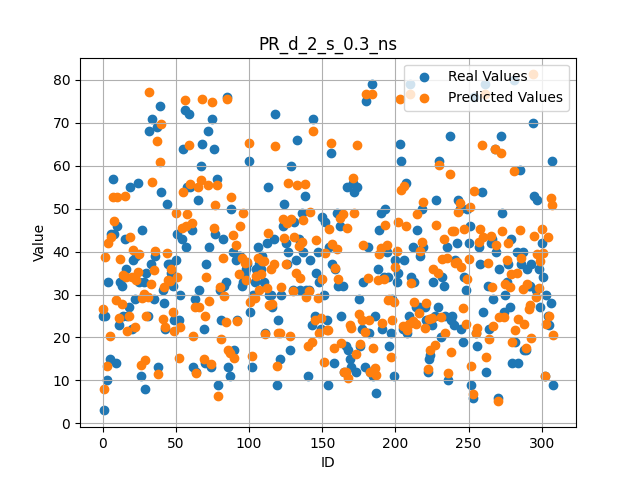
\includegraphics[width=0.9\textwidth]{graphics/plots/PR_d_2_s_0.3_ns.png} \\
		\caption{Wykres porównujący wartości rzeczywiste z przewidywanymi dla modelu PR\_d\_2\_s\_0.3\_ns}
	\end{center}
\end{itemize}
\\ \\
Model regresji wielomianowej stopnia 2 dla 50\% zbioru treningowego:
\begin{itemize}
	\item nazwa modelu: PR\_d\_2\_s\_0.5\_ns
	\item błąd średniokwadratowy: 66.36971163392116
	\item współczynnik determinacji: 0.7599499615396053
	\item walidacja krzyżowa dla cv=2: 0.6565261166365575
	\item walidacja krzyżowa dla cv=3: 0.754689342213766
	\item walidacja krzyżowa dla cv=4: 0.762473153465002
	\item wykres porównujący wartości rzeczywiste z wartościami przewidywanymi: \begin{center} \small
		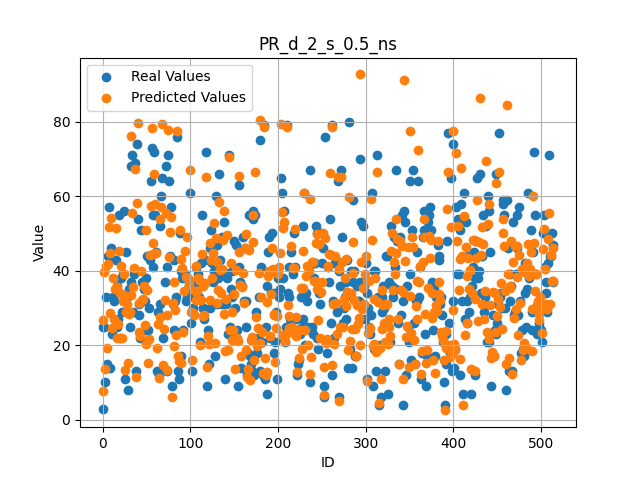
\includegraphics[width=0.9\textwidth]{graphics/plots/PR_d_2_s_0.5_ns.png} \\
		\caption{Wykres porównujący wartości rzeczywiste z przewidywanymi dla modelu PR\_d\_2\_s\_0.5\_ns}
	\end{center}
\end{itemize}
\\ \\
Model z wykorzystaniem RFE stopnia 2 o 8 cechach dla 30\% zbioru treningowego:
\begin{itemize}
	\item nazwa modelu: RFE\_d\_2\_nf\_8\_s\_0.3\_ns
	\item błąd średniokwadratowy: 79.12807052235767
	\item współczynnik determinacji: 0.7163791677007509
	\item walidacja krzyżowa dla cv=2: 0.5587452765381222
	\item walidacja krzyżowa dla cv=3: 0.6612126286969477
	\item walidacja krzyżowa dla cv=4: 0.5905217307658854
	\item wykres porównujący wartości rzeczywiste z wartościami przewidywanymi: \begin{center} \small
		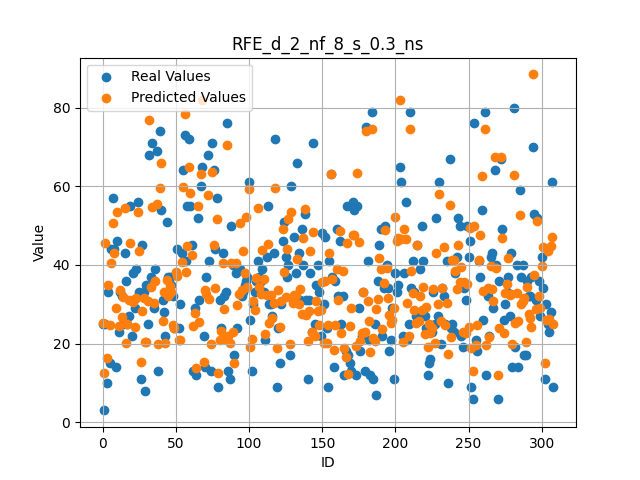
\includegraphics[width=0.9\textwidth]{graphics/plots/RFE_d_2_nf_8_s_0.3_ns.png} \\
		\caption{Wykres porównujący wartości rzeczywiste z przewidywanymi dla modelu RFE\_d\_2\_nf\_8\_s\_0.3\_ns}
	\end{center}
\end{itemize}
\\ \\
Wszystkie trzy modele mają współczynnik determinacji między 0.71 a 0.78, co oznacza, że modele są dość dobre.
Wartości walidacji krzyżowej dla cv o wartości 2, 3 i 4 są zbliżone dla wybranych modeli, co oznacza, że są one stabilne.
\subsection{Wyniki symulacji dla danych ze skalowaniem}
Na podstawie wygenerowanych modeli wybraliśmy trzy najlepsze z nich dla zbioru ze skalowaniem. Są to:
\begin{enumerate}
	\item Model regresji wielomianowej stopnia 2 dla 20\% zbioru treningowego
	\item Model regresji wielomianowej stopnia 2 dla 30\% zbioru treningowego
	\item Model regresji wielomianowej stopnia 2 dla 50\% zbioru treningowego
\end{enumerate}
\\ \\
Zostały one wybrane na podstawie tych samych wyznaczników jak w przypadku modeli wygenerowanych bez skalowania zbioru danych.
\\ \\
Model regresji wielomianowej stopnia 2 dla 20\% zbioru treningowego:
\begin{itemize}
	\item nazwa modelu: PR\_d\_2\_s\_0.2\_s
	\item błąd średniokwadratowy: 51.0119559547858
	\item współczynnik determinacji: 0.8174597501290759
	\item walidacja krzyżowa dla cv=2: 0.3020929003546536
	\item walidacja krzyżowa dla cv=3: 0.6135095033450021
	\item walidacja krzyżowa dla cv=4: 0.7070370517697293
	\item wykres porównujący wartości rzeczywiste z wartościami przewidywanymi: \begin{center} \small
		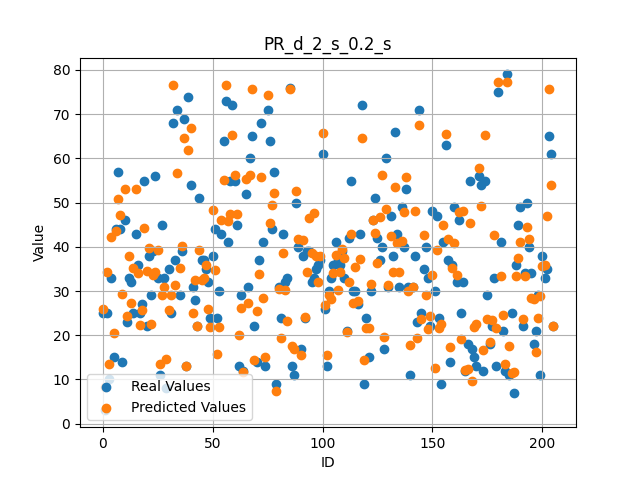
\includegraphics[width=0.9\textwidth]{graphics/plots/PR_d_2_s_0.2_s.png} \\
		\caption{Wykres porównujący wartości rzeczywiste z przewidywanymi dla modelu PR\_d\_2\_s\_0.2\_s}
	\end{center}
\end{itemize}
\\ \\
Model regresji wielomianowej stopnia 2 dla 30\% zbioru treningowego:
\begin{itemize}
	\item nazwa modelu: PR\_d\_2\_s\_0.3\_s
	\item błąd średniokwadratowy: 58.945251382045186
	\item współczynnik determinacji: 0.7887209792087575
	\item walidacja krzyżowa dla cv=2: 0.5837776709109881
	\item walidacja krzyżowa dla cv=3: 0.6956812085237528
	\item walidacja krzyżowa dla cv=4: 0.5081744180788107
	\item wykres porównujący wartości rzeczywiste z wartościami przewidywanymi: \begin{center} \small
		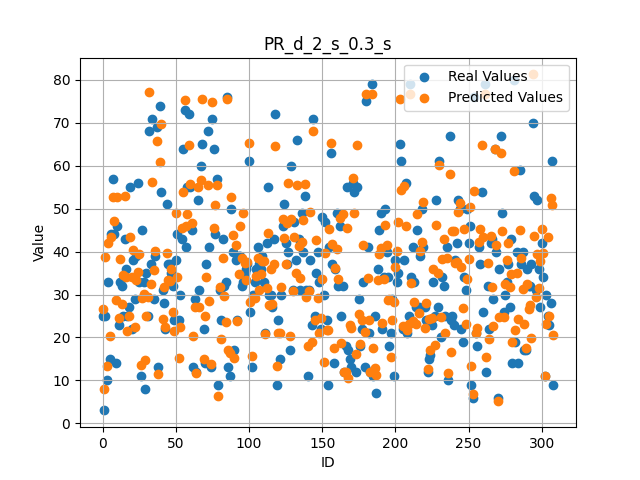
\includegraphics[width=0.9\textwidth]{graphics/plots/PR_d_2_s_0.3_s.png} \\
		\caption{Wykres porównujący wartości rzeczywiste z przewidywanymi dla modelu PR\_d\_2\_s\_0.3\_s}
	\end{center}
\end{itemize}
\\ \\
Model regresji wielomianowej stopnia 2 dla 50\% zbioru treningowego:
\begin{itemize}
	\item nazwa modelu: PR\_d\_2\_s\_0.5\_s
	\item błąd średniokwadratowy: 66.36971163441056
	\item współczynnik determinacji: 0.7599499615378352
	\item walidacja krzyżowa dla cv=2: 0.6987226149686151
	\item walidacja krzyżowa dla cv=3: 0.7546893422127049
	\item walidacja krzyżowa dla cv=4: 0.7624731534636663
	\item wykres porównujący wartości rzeczywiste z wartościami przewidywanymi: \begin{center} \small
		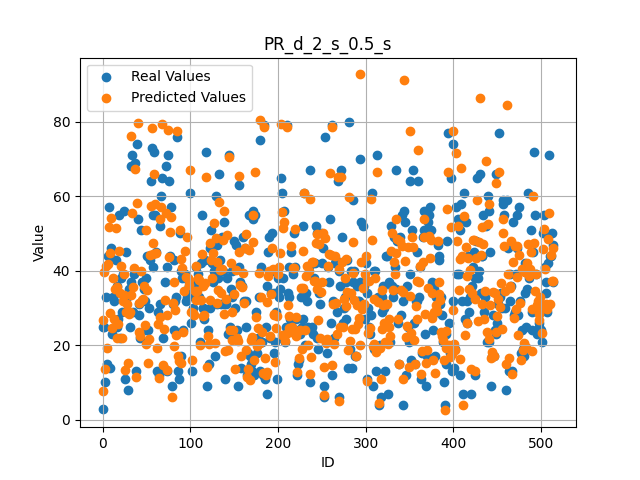
\includegraphics[width=0.9\textwidth]{graphics/plots/PR_d_2_s_0.5_s.png} \\
		\caption{Wykres porównujący wartości rzeczywiste z przewidywanymi dla modelu PR\_d\_2\_s\_0.5\_s}
	\end{center}
\end{itemize}
\\ \\
Wszystkie trzy modele mają współczynnik determinacji między 0.75 a 0.82, co oznacza, że modele są dość dobre. Warto zwrócić uwagę na fakt, że w przypadku skalowanych danych wszystkie 3 najlepsze modele są modelami regresji wielomianowej stopnia 2.
Różnią się one jedynie wielkością zbioru treningowego. W tym przypadku uzyskano też niższe wartości błędu średniokwadratowego niż w przypadku modeli bez skalowania.
\subsection{Wyniki symulacji dla modeli regresji liniowej}
Ponieważ żaden model regresji liniowej nie był na tyle dobry, aby znaleźć się wśród najlepszych modeli, a tego dotyczyło główne polecenie zadania, to postanowiliśmy wygenerować ranking tylko dla modeli regresji liniowej.
\\ \\
Trzy najlepsze modele dla zbioru bez skalowania danych:
\begin{enumerate}
	\item Model regresji liniowej dla 20\% zbioru treningowego
	\item Model regresji liniowej dla 30\% zbioru treningowego
	\item Model regresji liniowej dla 40\% zbioru treningowego
\end{enumerate}
\\ \\
Model regresji liniowej dla 20\% zbioru treningowego:
\begin{itemize}
	\item nazwa modelu: LR\_s\_0.2\_ns
	\item błąd średniokwadratowy: 100.67526042702907
	\item współczynnik determinacji: 0.6397454900482769
	\item walidacja krzyżowa dla cv=2: 0.6055998055170613
	\item walidacja krzyżowa dla cv=3: 0.6017776001163333
	\item walidacja krzyżowa dla cv=4: 0.5991471569663839
	\item wykres porównujący wartości rzeczywiste z wartościami przewidywanymi: \begin{center} \small
		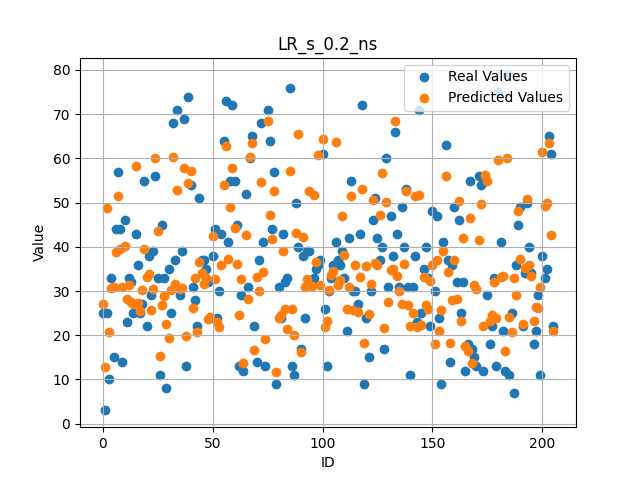
\includegraphics[width=0.9\textwidth]{graphics/plots/LR_s_0.2_ns.png} \\
		\caption{Wykres porównujący wartości rzeczywiste z przewidywanymi dla modelu LR\_s\_0.2\_ns}
	\end{center}
	\end{itemize}
\\ \\
Model regresji liniowej dla 30\% zbioru treningowego:
\begin{itemize}
	\item nazwa modelu: LR\_s\_0.3\_ns
	\item błąd średniokwadratowy: 105.69685723034375
	\item współczynnik determinacji: 0.6211479640386942
	\item walidacja krzyżowa dla cv=2: 0.6033683093006181
	\item walidacja krzyżowa dla cv=3: 0.6033559121495217
	\item walidacja krzyżowa dla cv=4: 0.5857841384745779
	\item wykres porównujący wartości rzeczywiste z wartościami przewidywanymi: \begin{center} \small
		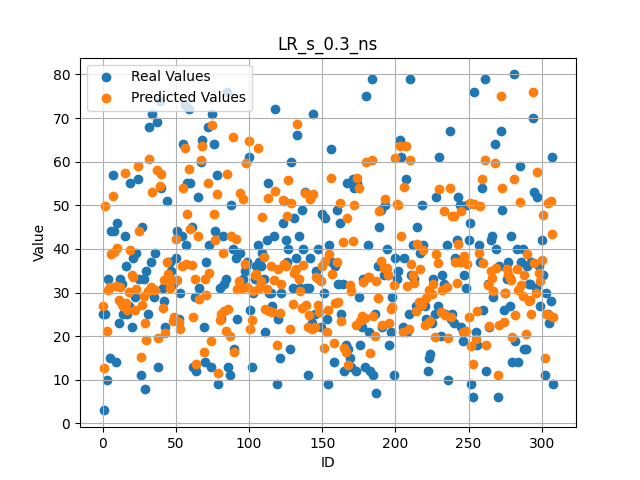
\includegraphics[width=0.9\textwidth]{graphics/plots/LR_s_0.3_ns.png} \\
		\caption{Wykres porównujący wartości rzeczywiste z przewidywanymi dla modelu LR\_s\_0.3\_ns}
	\end{center}
	\end{itemize}
\\ \\
Model regresji liniowej dla 40\% zbioru treningowego:
\begin{itemize}
	\item nazwa modelu: LR\_s\_0.4\_ns
	\item błąd średniokwadratowy: 106.25022155383516
	\item współczynnik determinacji: 0.6293974100833089
	\item walidacja krzyżowa dla cv=2: 0.612296554063505
	\item walidacja krzyżowa dla cv=3: 0.6192414216103493
	\item walidacja krzyżowa dla cv=4: 0.6224977912969356
	\item wykres porównujący wartości rzeczywiste z wartościami przewidywanymi: \begin{center} \small
		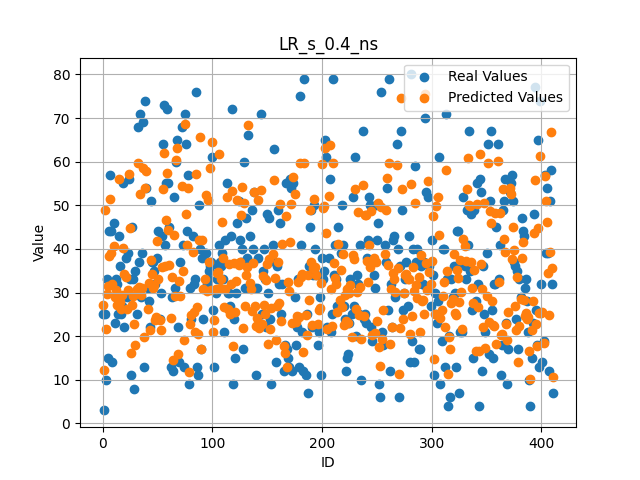
\includegraphics[width=0.9\textwidth]{graphics/plots/LR_s_0.4_ns.png} \\
		\caption{Wykres porównujący wartości rzeczywiste z przewidywanymi dla modelu LR\_s\_0.4\_ns}
	\end{center}
	\end{itemize}
\\ \\
Trzy najlepsze modele regresji liniowej dla zbioru ze skalowaniem danych:
\begin{enumerate}
	\item Model regresji liniowej dla 20\% zbioru treningowego
	\item Model regresji liniowej dla 30\% zbioru treningowego
	\item Model regresji liniowej dla 40\% zbioru treningowego
\end{enumerate}
\\ \\
Model regresji liniowej dla 20\% zbioru treningowego:
\begin{itemize}
	\item nazwa modelu: LR\_s\_0.2\_s
	\item błąd średniokwadratowy: 100.67526042702907
	\item współczynnik determinacji: 0.6397454900482769
	\item walidacja krzyżowa dla cv=2: 0.6055998055170614
	\item walidacja krzyżowa dla cv=3: 0.6017776001163332
	\item walidacja krzyżowa dla cv=4: 0.599147156966384
	\item wykres porównujący wartości rzeczywiste z wartościami przewidywanymi: \begin{center} \small
		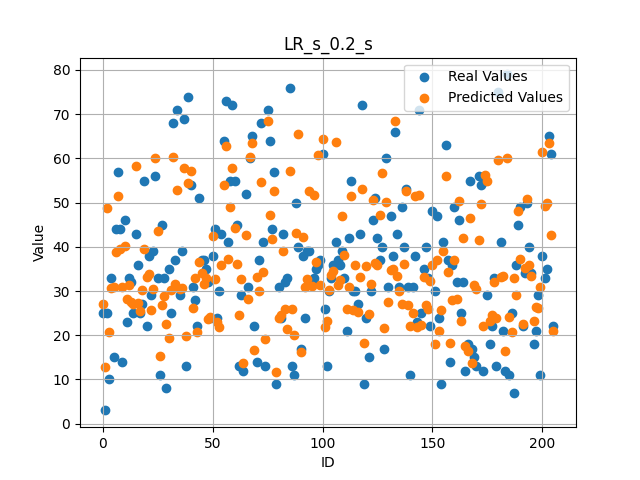
\includegraphics[width=0.9\textwidth]{graphics/plots/LR_s_0.2_s.png} \\
		\caption{Wykres porównujący wartości rzeczywiste z przewidywanymi dla modelu LR\_s\_0.2\_s}
	\end{center}
	\end{itemize}
\\ \\
Model regresji liniowej dla 30\% zbioru treningowego:
\begin{itemize}
	\item nazwa modelu: LR\_s\_0.3\_s
	\item błąd średniokwadratowy: 105.69685723034382
	\item współczynnik determinacji: 0.621147964038694
	\item walidacja krzyżowa dla cv=2: 0.6033683093006181
	\item walidacja krzyżowa dla cv=3: 0.6033559121495217
	\item walidacja krzyżowa dla cv=4: 0.5857841384745779
	\item wykres porównujący wartości rzeczywiste z wartościami przewidywanymi: \begin{center} \small
		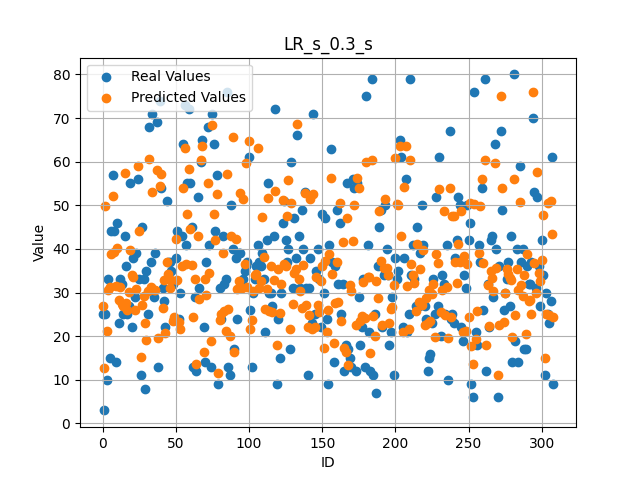
\includegraphics[width=0.9\textwidth]{graphics/plots/LR_s_0.3_s.png} \\
		\caption{Wykres porównujący wartości rzeczywiste z przewidywanymi dla modelu LR\_s\_0.3\_s}
	\end{center}
	\end{itemize}
\\ \\
Model regresji liniowej dla 40\% zbioru treningowego:
\begin{itemize}
	\item nazwa modelu: LR\_s\_0.4\_s
	\item błąd średniokwadratowy: 106.25022155383522
	\item współczynnik determinacji: 0.6293974100833086
	\item walidacja krzyżowa dla cv=2: 0.6122965540635052
	\item walidacja krzyżowa dla cv=3: 0.6192414216103493
	\item walidacja krzyżowa dla cv=4: 0.6224977912969356
	\item wykres porównujący wartości rzeczywiste z wartościami przewidywanymi: \begin{center} \small
		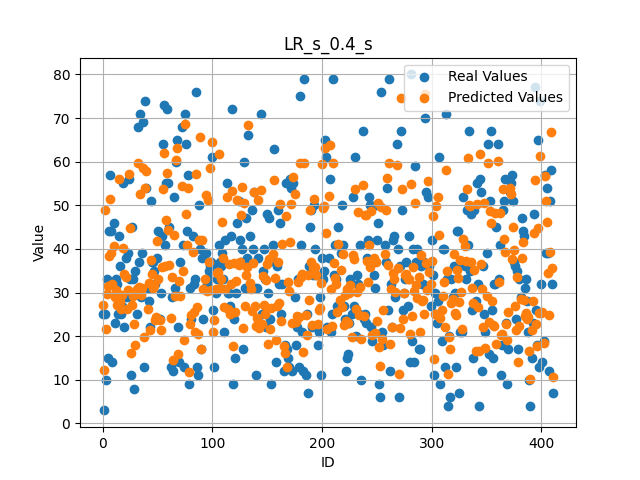
\includegraphics[width=0.9\textwidth]{graphics/plots/LR_s_0.4_s.png} \\
		\caption{Wykres porównujący wartości rzeczywiste z przewidywanymi dla modelu LR\_s\_0.4\_s}
	\end{center}
	\end{itemize}
\\ \\
Powyższe modele uzyskały podobne wartości błędu średniokwadratowego, który w każdym przypadku wyniósł wartość większą niż 100.
Wartość współczynnika determinacji również nie jest zadowalająca, ponieważ w każdym przypadku jest mniejsza niż 0.7. \\
Warto zwrócić uwagę na fakt, że w przypadku tych modeli zwiększenie rozmiaru zbioru treningowego nie wpłynęło na poprawę jakości modeli.
\subsection{Porównanie wyników uzyskanych przez modele}
Po porównaniu metryk uzyskanych przez najlepsze modele dla zbioru bez skalowania i ze skalowaniem można stwierdzić, że modele dla zbioru ze skalowaniem są lepsze.
Uzyskano znacznie niższe wartości błędu średniokwadratowego, gdzie jednocześnie wartości współczynnika determinacji są minimalnie wyższe.
Warto zwrócić uwagę na fakt, że 5 na 6 najlepszych modeli stanowią modele regresji wielomianowej stopnia 2. Niestety nie udało się uzyskać modelu regresji liniowej, który dorównałby tym modelom.
\\ \\
W przypadku najlepszych modeli regresji liniowej wyznaczone metryki, tj. błąd średniokwadratowy i współczynnik determinacji, są bardzo zbliżone.
Można więc stwierdzić, że w przypadku regresji liniowej nie ma znaczącej różnicy między skalowaniem i nie skalowaniem danych.
W porównaniu do regresji wielomianowej stopnia 2, regresja liniowa jest znacznie gorsza (dla badanego zbioru danych). Widać to zwłaszcza po uzyskanych wartościach współczynnika determinacji.
\subsection{Uwagi}
W wielu przypadkach po wyznaczeniu walidacji krzyżowej dla cv od 2 do 4 otrzymywaliśmy ujemne wartości. Możliwe, że jest to związane z tym, iż w danym przypadku model był zbyt złożony lub zbyt prosty dla wybranych danych.
Skutkuje to tym, że model nie jest w stanie dobrze przewidywać wartości dla zbioru testowego.
\chapter{Podsumowanie}
W pracy zostały przedstawione wyniki badań nad trenowaniem modeli regresji dla zbioru danych dotyczącego odporności betonu na ściskanie.
W sumie wygenerowano i porównano 112 modeli, wykorzystując metody regresji liniowej, wielomianowej z zastosowaniem Polynomial Features oraz algorytmu Recursive Feature Elimination. \\
Modele zostały porównane na podstawie wartości błędu średniokwadratowego oraz współczynnika determinacji. Najlepsze wyniki uzyskano dla modeli regresji wielomianowej stopnia 2.
Żaden model regresji liniowej nie był na tyle dobry, aby dorównać modelom regresji wielomianowej. \\
Najlepszy model regresji liniowej uzyskał wartość współczynnika determinacji równą zaledwie 0.63,
gdzie najlepszy model regresji wielomianowej stopnia 2 uzyskał wartość współczynnika determinacji równą 0.81.
Jest to znaczna różnica, dlatego w przypadku tego zbioru danych lepiej rozważyć inną metodę uczenia maszynowego niż algorytm regresji liniowej. \\
Modele trenowane na podstawie skalowanych danych uzyskały lepsze wyniki niż modele trenowane na podstawie nie skalowanych danych, co było spodziewanym rezultatem.
Różnice te nie były aż tak widoczne w przypadku modeli regresji liniowej, jednak mimo wszystko warto było przeprowadzić skalowanie danych. \\
Ciekawym zjawiskiem było to, że część modeli uzyskała ujemne wartości po przeprowadzeniu walidacji krzyżowej. Skutkowało to tym, że model nie był w stanie dobrze przewidywać wartości dla zbioru testowego. \\

\begin{appendices}
\chapter{Dane modeli}
\section{Pliki CSV z metrykami modeli}
Pliki CSV z metrykami modeli znajdują się w folerze \texttt{załączniki}. Nazwy plików to non\_scaled\_results.csv i scaled\_results.csv.
\section{Wygenerowane wykresy porównujące wartości rzeczywiste z przewidywanymi}
Wszystkie wykresy wygenerowane dla modeli znajdują się w folderze \texttt{graphics/plots}.
\chapter{Kod programu}
Link do repozytorium: \href{https://github.com/kjez21/KWD-Concrete}{KWD-Concrete} \\ \\
\begin{verbatim}
import csv
import pandas as pd
import numpy as np
from sklearn.preprocessing import StandardScaler
from sklearn.model_selection import train_test_split
from sklearn.linear_model import LinearRegression
from matplotlib import pyplot as plt
from sklearn.metrics import mean_squared_error
from sklearn.metrics import r2_score
from sklearn.model_selection import cross_val_score
import seaborn as sb
from scipy import stats
from sklearn.preprocessing import PolynomialFeatures
from sklearn.feature_selection import RFE


def importData():
    df = pd.read_excel(r'Concrete_Data.xls')
    pd.set_option('display.max_columns', None)
    print("Dataframe description:")
    print(df.describe())
    print("Dataframe head:")
    print(df.head())
    data = df.iloc[1:, 0:-1]
    target = df.iloc[1:, -1]

    return data, target, df


def analizeData(target, df, data_np):
    print("Value counts:")
    print(target.value_counts())
    sb.displot(target)
    plt.savefig("plots/target_distribution.png")
    plt.show()
    stats.probplot(target,
                   plot=plt) # Note: The target variable is not normally distributed, but it is close to normal distribution
    plt.savefig("plots/probplot.png")
    plt.show()
    targetLog = np.log(target)
    stats.probplot(targetLog, plot=plt)  # Note: log transformation seems to be worse
    plt.savefig("plots/log_probplot.png")
    plt.show()
    sb.pairplot(df)
    plt.savefig("plots/pairplot.png")
    plt.show()
    print("HeatMap")
    createHeatMap(df)
    print("Number of NULL values in each column:")
    print(df.isnull().sum())
    plt.boxplot(data_np)
    plt.savefig("plots/boxplot.png")
    plt.show()
    print('---Mean---')
    print(data_np.mean(axis=0))
    print('--std---')
    print(data_np.std(axis=0))


def createHeatMap(df):
    correlation_matrix = df.corr().round(2)
    print("Correlation matrix:")
    print(correlation_matrix)
    sb.heatmap(data=correlation_matrix,
               annot=True)  # Note: The strongest correlation is between cement and compressive strength
    # Note: the heatmap confirms the results from the pairplot
    plt.savefig("plots/heatmap.png", bbox_inches='tight')
    plt.show()


def convertToNpArray(data, target):
    data_np = np.array(data, dtype=np.int16)
    target_np = np.array(target, dtype=np.int16)

    print(data_np.shape)
    print(target_np.shape)
    return data_np, target_np


def scaleData(data):
    scaler = StandardScaler()
    scaled_data = scaler.fit_transform(data)
    print(scaled_data[1, :])
    print('---Mean---')
    print(scaled_data.mean(axis=0))
    print('--std---')
    print(scaled_data.std(axis=0))
    return scaled_data


def splitData(data, target, size):
    train_data, test_data, \
    train_target, test_target = \
        train_test_split(data, target, test_size=size, random_state=10)

    print("Training dataset:")
    print("train_data:", train_data.shape)
    print("train_target:", train_target.shape)
    print("Testing dataset:")
    print("test_data:", test_data.shape)
    print("test_target:", test_target.shape)
    return train_data, test_data, train_target, test_target


def trainLinearRegressionModel(train_data, train_target):
    linear_regression = LinearRegression()
    linear_regression.fit(train_data, train_target)
    return linear_regression


def getPredictedValues(linear_regression, test_data, test_target):
    realValues = []
    predictedValues = []
    ids = []
    for x in range(0, len(test_data)):
        prediction = linear_regression.predict(test_data[x, :].reshape(1, -1))
        realValues.append(test_target[x])
        predictedValues.append(prediction)
        ids.append(x)

    return realValues, predictedValues, ids


def createPlot(arr1, arr2, title):
    plt.scatter(arr1['ids'], arr1['arr'], label=arr1['label'])
    plt.scatter(arr2['ids'], arr2['arr'], label=arr2['label'])
    plt.title(title)
    plt.xlabel('ID')
    plt.ylabel('Value')
    plt.legend()
    plt.grid(True)
    plt.savefig("plots/" + title + ".png")
    plt.show()


def prepDict(arr, ids, label):
    return {
        'arr': arr,
        'ids': ids,
        'label': label
    }


def crossValidate(data, target, cv):
    scores = cross_val_score(LinearRegression(), data, target, cv=cv)
    print(scores)
    print(scores.mean())
    return scores.mean()


def polynomialFeatures(trainData, testData, trainTarget, degree):
    poly = PolynomialFeatures(degree)
    trainDataPoly = poly.fit_transform(trainData)
    testDataPoly = poly.fit_transform(testData)
    lr_poly = LinearRegression()
    lr_poly.fit(trainDataPoly, trainTarget)
    return lr_poly, trainDataPoly, testDataPoly


def reduceFeatures(trainData, testData, trainTarget, degree,
                   numOfFeatures):  # Note: degree = 1 -> without polynomial features
    lr_poly, trainDataPoly, testDataPoly = polynomialFeatures(trainData, testData, trainTarget, degree)
    rfe = RFE(lr_poly, n_features_to_select=numOfFeatures)
    rfe = rfe.fit(trainDataPoly, trainTarget)
    print(rfe.support_)
    print(rfe.ranking_)
    return rfe, trainDataPoly, testDataPoly


def validateModel(data, target, model, name):
    realValues, predictedValues, ids = getPredictedValues(model, data, target)
    print("Mean squared error of a learned model: ", mean_squared_error(realValues, predictedValues))
    print('Variance score: ', r2_score(realValues, predictedValues))
    cv = []
    for x in range(2, 5):
        cv.append({
            'cv': x,
            'score': crossValidate(data, target, x)
        })
    realValsDict = prepDict(realValues, ids, "Real Values")
    predictedValsDict = prepDict(predictedValues, ids, "Predicted Values")
    createPlot(realValsDict, predictedValsDict, name)
    return {
        'mean': mean_squared_error(realValues, predictedValues),
        'variance': r2_score(realValues, predictedValues),
        'cv': cv
    }


def trainModels(data, target, postfix):
    dataSizes = [0.2, 0.3, 0.4, 0.5]

    results = []
    for size in dataSizes:
        models = []
        train_data, test_data, train_target, test_target = splitData(data, target, size)

        lrModel = trainLinearRegressionModel(train_data, train_target)
        models.append({
            'model': lrModel,
            'testData': test_data,
            'dataSize': size,
            'name': 'LR_s_' + str(size) + "_" + postfix,
            'type': 'LR'
        })

        for degree in range(2, 5):
            lrPolyModel, trainDataPoly, testDataPoly = polynomialFeatures(train_data, test_data, train_target, degree)
            models.append({
                'model': lrPolyModel,
                'testData': testDataPoly,
                'degree': degree,
                'dataSize': size,
                'name': 'PR_d_' + str(degree) + "_s_" + str(size) + "_" + postfix,  # Polynomial Regression Model
                'type': 'PR'
            })

        # Note: degree = 2 -> the best model for this dataset
        for numOfFeatures in range(5, 15):
            rfe, trainDataPoly, testDataPoly = reduceFeatures(train_data, test_data, train_target, 2, numOfFeatures)
            models.append({
                'model': rfe,
                'testData': testDataPoly,
                'numOfFeatures': numOfFeatures,
                'dataSize': size,
                'name': 'RFE_d_2_nf_' + str(numOfFeatures) + "_s_" + str(size) + "_" + postfix,
                'type': 'RFE'
            })

        for model in models:
            print(model['name'])
            results.append({
                'model': model,
                'validation': validateModel(model['testData'], test_target, model['model'], model['name'])
            })

    return results


def printModelsResults(results):
    for result in results:
        print(result['model']['name'])
        print("Mean squared error: ", result['validation']['mean'])
        print("Variance score: ", result['validation']['variance'])
        print("Cross Validation: ")
        for cv in result['validation']['cv']:
            print("CV: ", cv['cv'], " Score: ", cv['score'])
        print("")


def saveModelsResultsToCSV(results, filename):
    with open(filename, 'w') as csvfile:
        fieldnames = ['name', 'mean', 'variance', 'cv2', 'cv3', 'cv4']
        writer = csv.DictWriter(csvfile, fieldnames=fieldnames)
        writer.writeheader()
        for result in results:
            writer.writerow({
                'name': result['model']['name'],
                'mean': result['validation']['mean'],
                'variance': result['validation']['variance'],
                'cv2': result['validation']['cv'][0]['score'],
                'cv3': result['validation']['cv'][1]['score'],
                'cv4': result['validation']['cv'][2]['score']
            })


def chooseBestModel(results):
    bestModel = results[0]
    for result in results:
        if result['validation']['mean'] >= bestModel['validation']['mean']:
            continue
        if result['validation']['variance'] <= bestModel['validation']['variance']:
            continue
        if result['validation']['cv'][0]['score'] <= 0:
            continue
        if result['validation']['cv'][1]['score'] <= 0:
            continue
        if result['validation']['cv'][2]['score'] <= 0:
            continue
        bestModel = result
    return bestModel


def getNBestModels(results, n):
    bestModels = []
    for i in range(0, n):
        bestModel = chooseBestModel(results)
        bestModels.append(bestModel)
        results.remove(bestModel)
    return bestModels


def getNBestLRModels(results, n):
    lrModels = []
    for result in results:
        if result['model']['type'] == 'LR':
            lrModels.append(result)
    bestModels = []
    for i in range(0, n):
        bestModel = chooseBestModel(lrModels)
        if bestModel['model']['type'] != 'LR':
            continue
        bestModels.append(bestModel)
        lrModels.remove(bestModel)
    return bestModels


def init():
    data, target, df = importData()
    data_np, target_np = convertToNpArray(data, target)
    analizeData(target, df, data_np)

    results = trainModels(data_np, target_np, 'ns')
    scaledResults = trainModels(scaleData(data_np), target_np, 's')

    print("Results:")
    print(results)
    print("Scaled results:")
    print(scaledResults)
    saveModelsResultsToCSV(results, 'non-scaled_results.csv')
    saveModelsResultsToCSV(scaledResults, 'scaled_results.csv')
    printModelsResults(results)
    printModelsResults(scaledResults)

    bestModel = chooseBestModel(results)
    print("Best model for non-scaled data: ", bestModel['model']['name'])
    printModelsResults([bestModel])

    bestModel = chooseBestModel(scaledResults)
    print("Best model for scaled data: ", bestModel['model']['name'])
    printModelsResults([bestModel])

    bestModelsScaled = getNBestModels(scaledResults, 3)
    print("Best models for scaled data: ")
    printModelsResults(bestModelsScaled)
    bestModelsNonScaled = getNBestModels(results, 3)
    print("Best models for non-scaled data: ")
    printModelsResults(bestModelsNonScaled)

    bestLRModelsScaled = getNBestLRModels(scaledResults, 3)
    print("Best LR models for scaled data: ")
    printModelsResults(bestLRModelsScaled)
    bestLRModelsNonScaled = getNBestLRModels(results, 3)
    print("Best LR models for non-scaled data: ")
    printModelsResults(bestLRModelsNonScaled)

init()

\end{verbatim}
\end{appendices}

\end{document}